\documentclass[11pt]{article}
\newcommand\tab[1][1cm]{\hspace*{#1}}
\usepackage{graphicx}
\graphicspath{ {C:/Users/yedkk/Desktop/CS465/hw4} }
\begin{document}
\section{Homework 4}
Name: Kangdong Yuan
	
\subsection{problem1}
a).I did not work in a group.
\\b).I did not consult without anyone my group members
\\c).I did not consult any non-class materials.

\subsection{problem2}
First we need to count the number of vertices $|V|$ in this graph G. We count the number of edge in this graph by dfs or bfs. if the count of edges exceed $|V|-1$, return yes. If there are only $|V|-1$ edges in graph G, we return no.  \\
The time to count vertices is $|V|$, and the time to count $|V|$ edges is $O(|V|)$. So, the time complexity of this algorithm is $2|V|=O(|V|)$ 

\subsection{problem3}
a). the minimum spanning tree will not change\\
\\the reason behind it: if graph has n vertices, then any spanning tree of G has $n-1$ edges. We define the cost of each spanning tree are $x_1,x_2,x_3,...x_j$. If each edge's weight decrease by 1, the cost of every spanning tree will decrease  by a constant $n-1$. So, the new cost of each spanning tree are $x_1-(n-1),x_2-(n-1),x_3-(n-1),...x_j-(n-1)$. Thus, the order of cost of spanning trees will not change, so the mst will still be the mst in new graph after weight changing.   \\
\\
b).but the shortest path may change\\
for example, this is the original graph, the shortest path from vertex 1 to vertex 2 is edge(1,2)\\
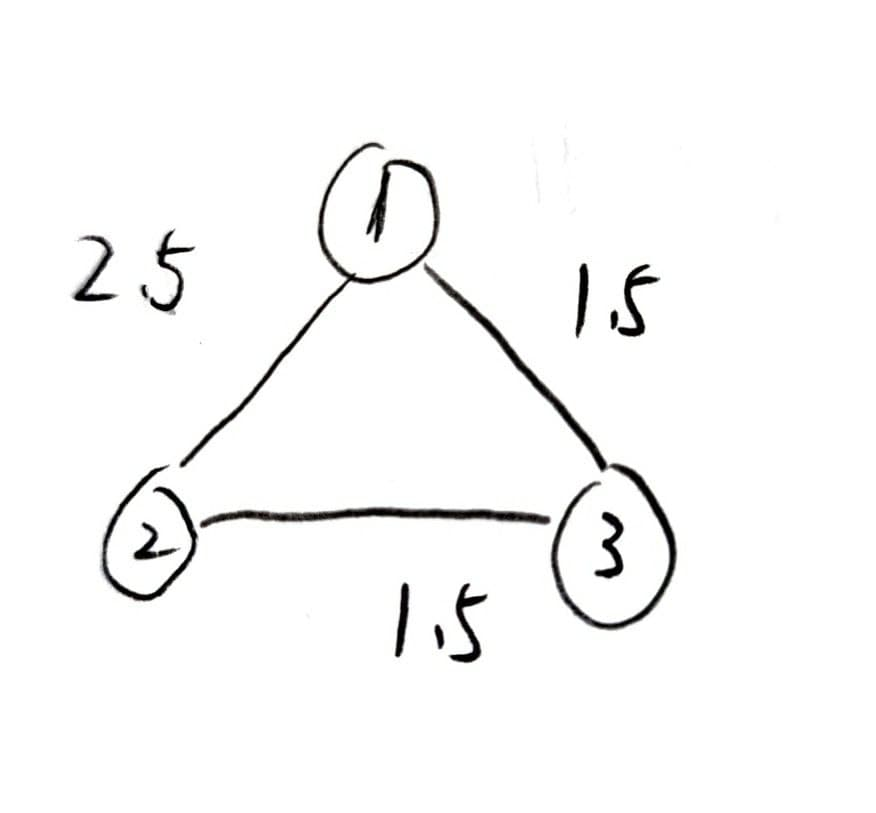
\includegraphics[scale=0.2]{og1}\\
This is the new graph that all edge weights minus 1, the shortest path from vertex 1 to vertex 2 is edge (1,3), (3,2)\\
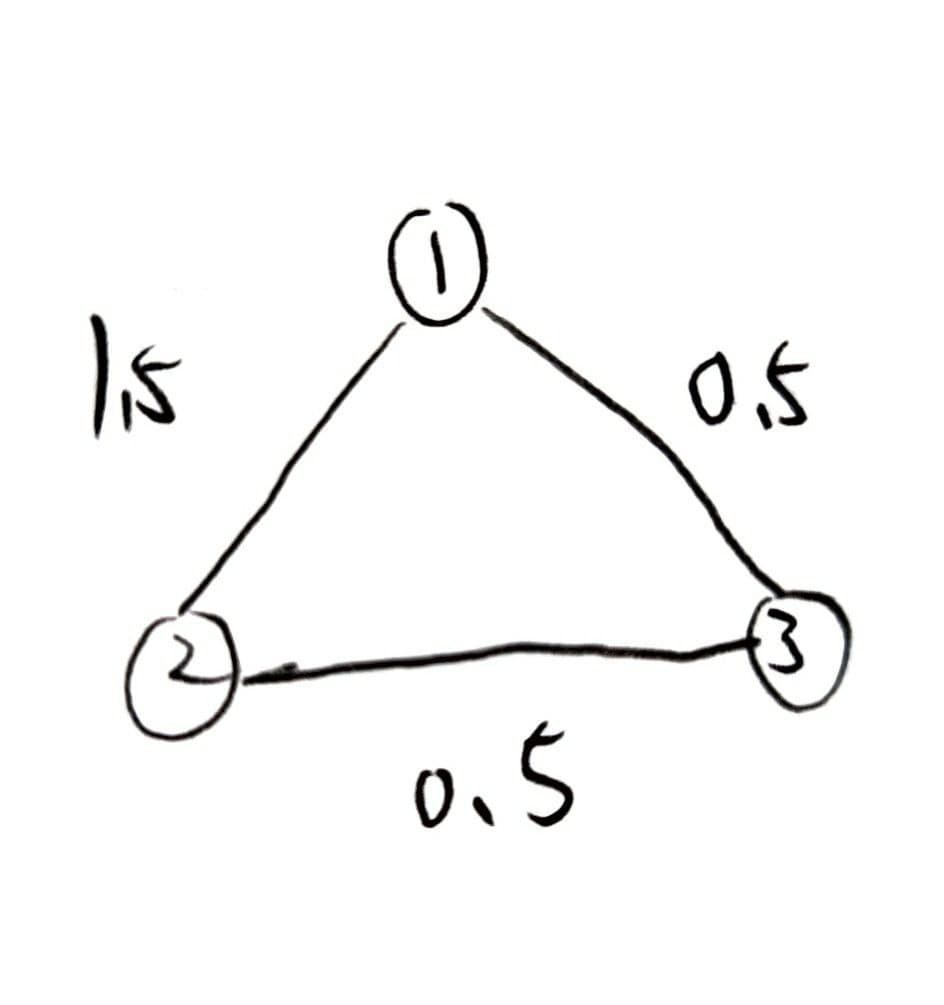
\includegraphics[scale=0.2]{ng1}\\
so the shortest path may change after edge weights changed\\
\subsection{problem4}
we prove by the contradiction.\\
Suppose this claim not hold, which is $T\cap U \notin T_H$. Then there is an edge $e\in T \cap H$ across some cut $(S|V-S)$ of H such that another edge across the cut, where the weight $e'$ is less. However, H is a subgraph of G, so $e'$ is lighter edge than e across the cut $(S|V-S)$ of G. This new edge $e$ should replace the edge in minimum spanning tree in G because it provide less cost, contradicting that T is an MST.








\end{document}